\documentclass[11pt]{article}

\usepackage[T1]{fontenc}
\usepackage[utf8]{inputenc}
\usepackage{lmodern}
\usepackage{microtype}
\usepackage{geometry}
\geometry{margin=1in}
\usepackage{amsmath}
\usepackage{amssymb}
\usepackage{mathtools}
\usepackage{graphicx}
\usepackage{subcaption}
\usepackage{booktabs}
\usepackage{multirow}
\usepackage{array}
\usepackage{tabularx}
\usepackage{longtable}
\usepackage{hyperref}
\usepackage{cleveref}
\usepackage{xcolor}

\title{Reconocimiento de Morfologias Hematologicas No Vistas en Regimen Open-Set bajo Cambio de Dominio}
\author{G. Álvarez Sánchez}
\date{}

\begin{document}
\maketitle

\begin{abstract}
El reconocimiento open-set es un requisito central pero poco evaluado en clasificadores de imagen hematologica: un modelo entrenado con una taxonomia fija puede encontrar morfologias fuera de esa taxonomia y, aun asi, verse obligado a asignar cada imagen a una clase conocida. Evaluamos este problema con un protocolo congelado y reproducible para reconocimiento morfologico de leucocitos. El dominio interno fue MLL23, con 41,621 imagenes unicelulares, cinco clases conocidas de leucocitos maduros y 13 morfologias desconocidas retenidas solo para evaluacion. En cinco semillas y dos protocolos de particion, los clasificadores ResNet18 alcanzaron macro-F1 closed-set cercano a 0.97, pero el rendimiento open-set fue menos robusto. CE+ViM obtuvo AUROC 0.877 $\pm$ 0.004 en V1 y 0.874 $\pm$ 0.008 en V2; sin embargo, su ventaja no se transfirio al dominio externo. En AML-LMU, un conjunto independiente de 18,365 imagenes usado solo como prueba, todos los sistemas principales degradaron: el AUROC externo estuvo entre 0.563 y 0.696 para sistemas V1 y entre 0.573 y 0.696 para sistemas V2, con FPR@95TPR alto. El orden de los metodos post-hoc cambio bajo cambio de dominio, con MSP superando a ViM externamente en las comparaciones principales. El analisis de fallos mostro fuerte dependencia morfologica, incluyendo rechazo dificil de neutrofilo en banda, monoblasto, mieloblasto, linfocito atipico y celula sombra. ArcFace mejoro algunas metricas geometricas de clases conocidas, pero fallo la confirmacion multisemilla/split como representacion superior robusta. La homologia persistente cubical y la topologia Vietoris-Rips fueron informativas como analisis negativo y explicativo, respectivamente, pero no como predictores confirmados de rendimiento open-set.
\end{abstract}

\section{Introduccion}

El reconocimiento automatico de morfologia leucocitaria suele formularse como clasificacion closed-set: cada imagen evaluada se asume perteneciente a una de las clases observadas durante el entrenamiento. Bajo esa formulacion, redes convolucionales modernas pueden lograr desempeno alto en conjuntos unicelulares curados. Sin embargo, esa evaluacion no responde una pregunta mas dificil. Un sistema entrenado para distinguir una taxonomia fija de leucocitos maduros puede encontrar celulas inmaduras, atipicas, raras o fuera de taxonomia durante la prueba. En ese escenario, forzar cada entrada hacia la clase conocida mas cercana puede ocultar fallos relevantes del protocolo experimental.

Este trabajo estudia reconocimiento open-set para morfologia hematologica. La taxonomia conocida contiene cinco clases de leucocitos maduros: basofilo, eosinofilo, linfocito, monocito y neutrofilo segmentado. Todas las demas morfologias evaluadas son desconocidas solo en sentido protocolario: estan fuera de la taxonomia de entrenamiento conocida. Esta definicion es estrecha e intencional. Una muestra desconocida no es una etiqueta de cancer, leucemia, malignidad, diagnostico ni positividad clinica. La tarea no es diagnosticar enfermedad, sino evaluar si un clasificador entrenado con una taxonomia conocida puede reconocer que una imagen no deberia ser forzada dentro de esa taxonomia.

La distincion importa porque la clasificacion closed-set y el rechazo de desconocidos miden comportamientos diferentes. Un modelo puede aprender representaciones compactas para clases conocidas y aun asi ubicar una morfologia no vista cerca de una clase conocida semanticamente relacionada. Por ejemplo, un neutrofilo en banda puede ser cercano a neutrofilos segmentados, y morfologias linfoides no vistas pueden ser atraidas hacia la clase linfocito. Este patron puede mantener alta la exactitud closed-set mientras la confiabilidad open-set sigue siendo limitada.

El estudio se plantea como evaluacion reproducible, no como afirmacion de un metodo nuevo superior. El dominio interno es MLL23, un conjunto grande de sangre periferica unicelular anotado por expertos \cite{mll23_nature_2025,mll23_zenodo_2024}. La validacion externa usa AML-Cytomorphology\_LMU, una coleccion independiente de TCIA con 18,365 imagenes unicelulares \cite{aml_lmu_tcia_2019}. AML-LMU se usa exclusivamente como prueba externa: no hay ajuste fino externo, calibracion externa de umbrales, ajuste externo de ViM, seleccion externa de metodo ni cambio de taxonomia.

La contribucion principal es una evaluacion reproducible y disciplinada de reconocimiento open-set hematologico bajo sensibilidad a semillas, sensibilidad a particiones, cambio de dominio externo y fallos dependientes de morfologia. Las contribuciones secundarias son: una comparacion sistematica de scores OSR post-hoc y aprendizaje de representaciones; un analisis de fallos morfologicos mediante atractores hacia clases conocidas; y un analisis geometrico/topologico explicativo de embeddings aprendidos.

\begin{figure}[htbp]
\centering
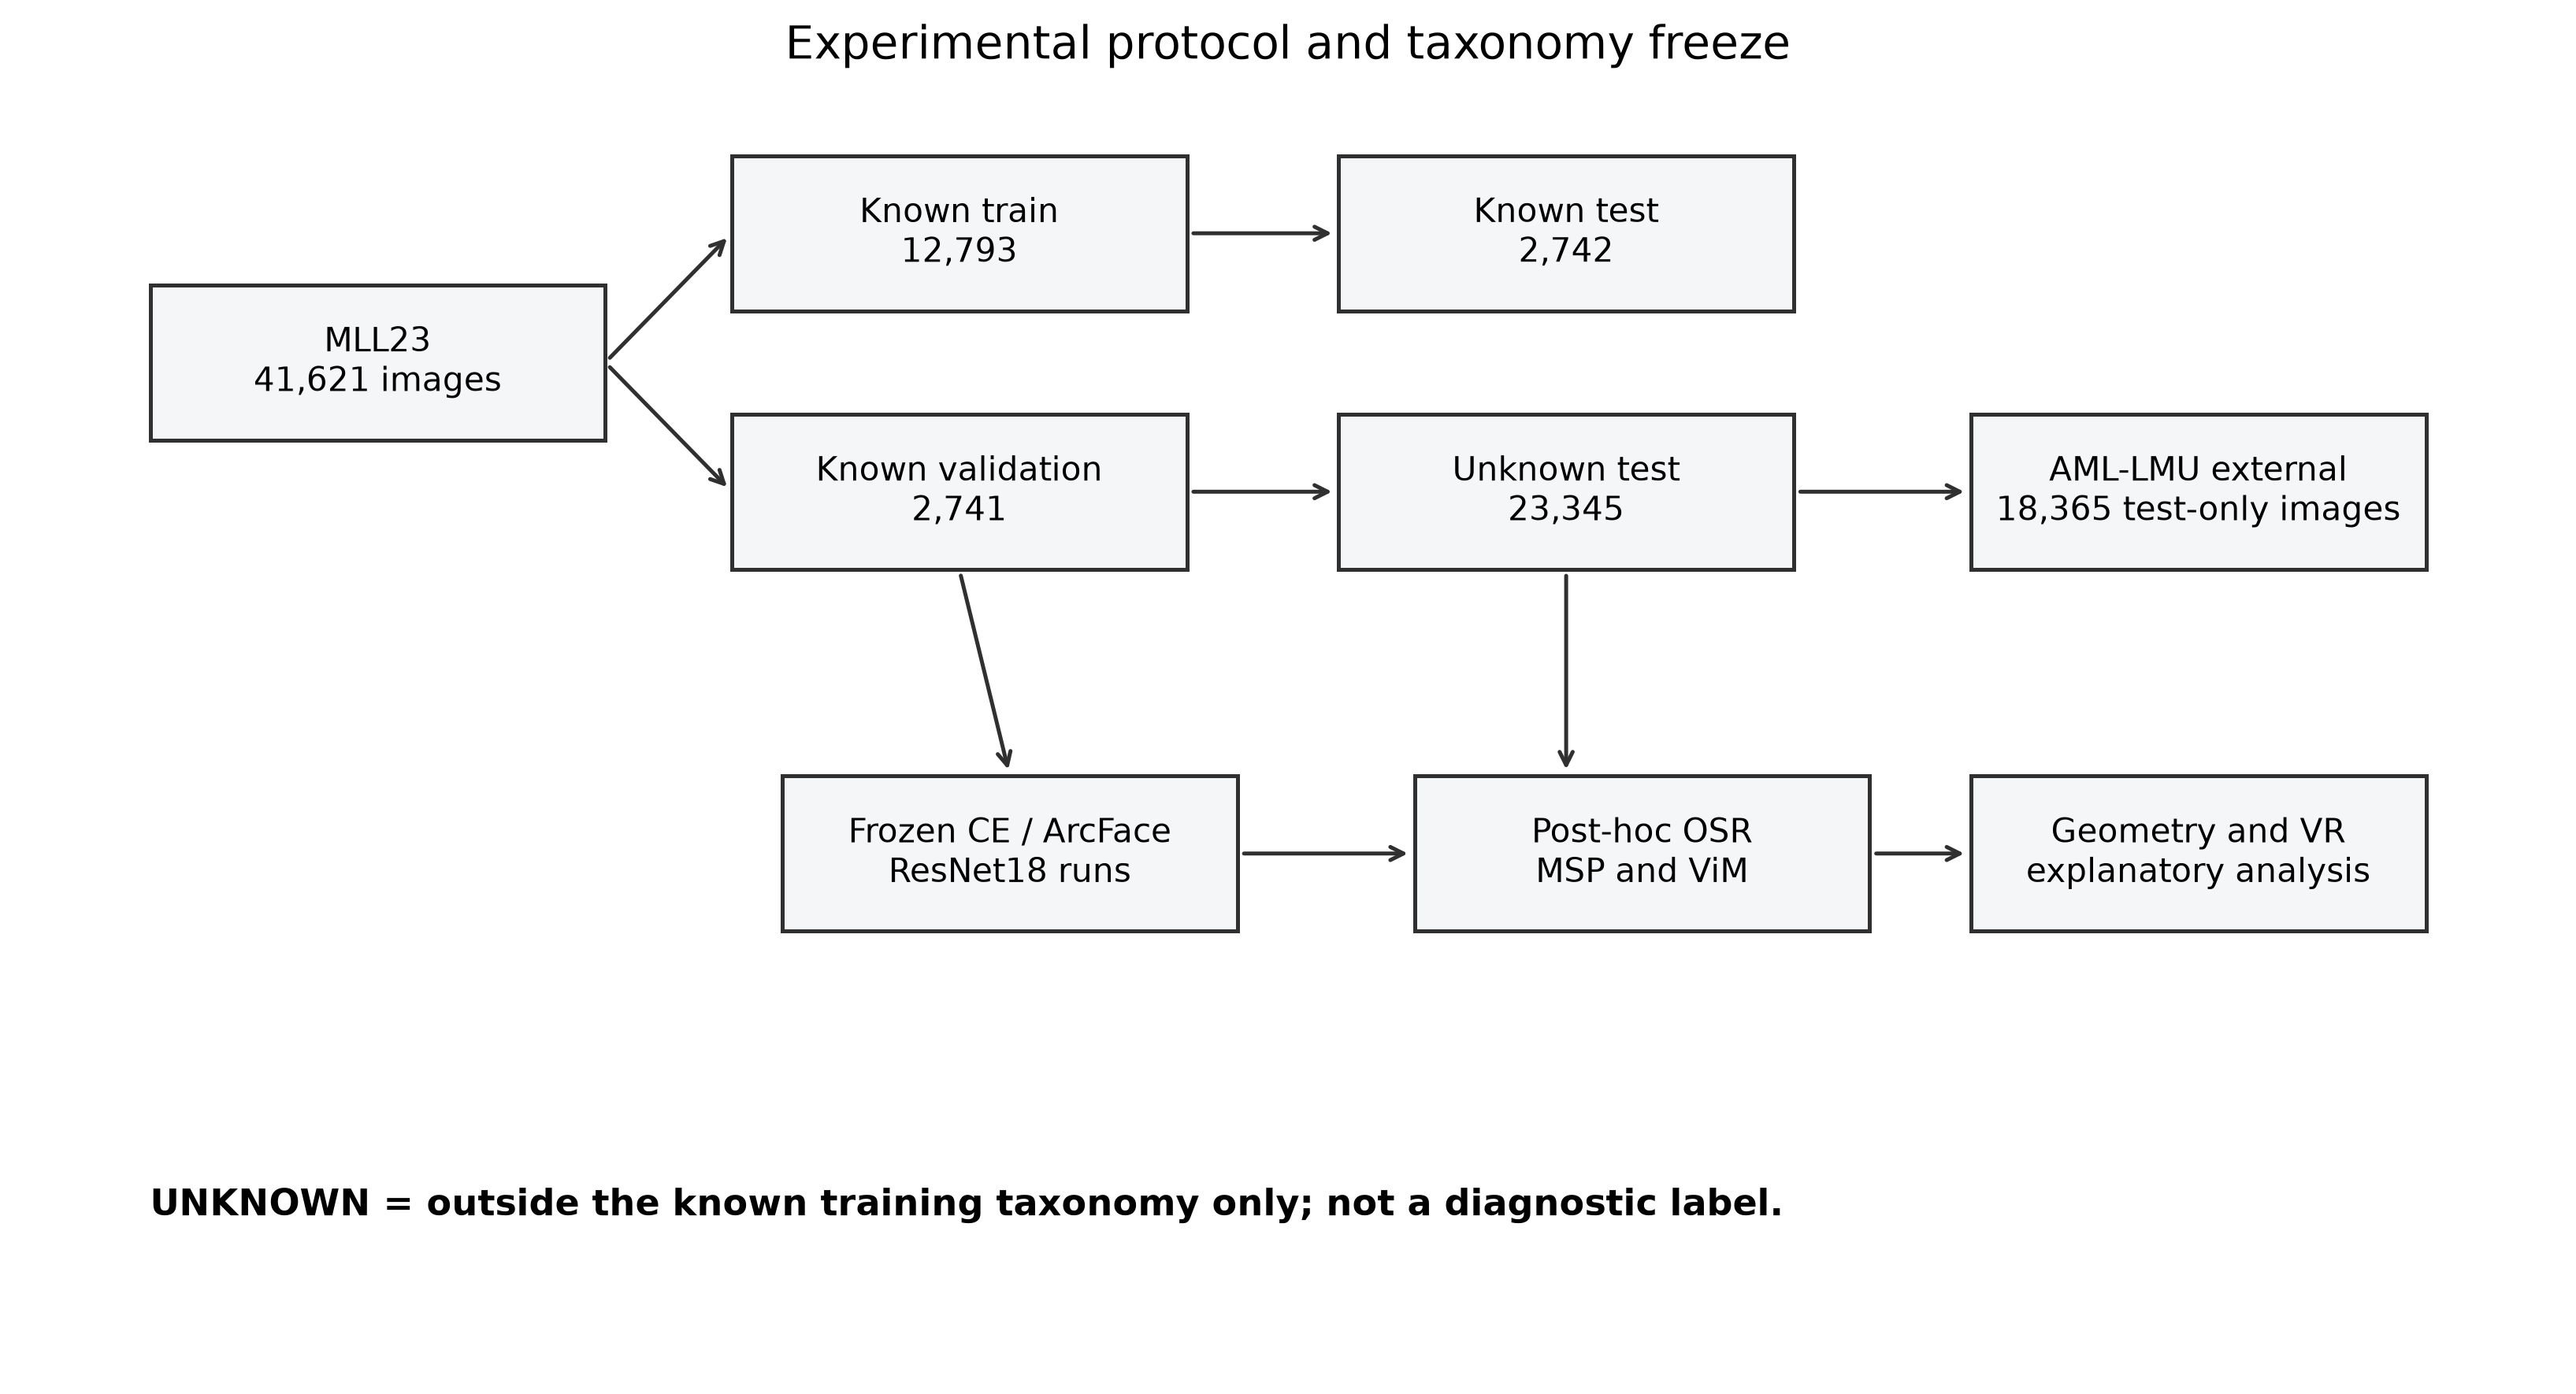
\includegraphics[width=\textwidth]{figures/figure1_protocol.png}
\caption{Protocolo congelado de evaluacion open-set. MLL23 se usa para evaluacion interna multisemilla y sensibilidad V1/V2; AML-LMU se usa como dominio externo solo de prueba.}
\label{fig:protocolo-es}
\end{figure}

\section{Trabajo Relacionado}

El aprendizaje profundo se ha usado ampliamente para clasificacion de celulas sanguineas, normalmente bajo una configuracion closed-set en la que todas las clases de prueba aparecen durante entrenamiento. MLL23 ofrece un recurso reciente de gran escala para morfologia unicelular en sangre periferica \cite{mll23_nature_2025,mll23_zenodo_2024}. AML-LMU proporciona un dominio independiente con imagenes unicelulares etiquetadas por expertos \cite{aml_lmu_tcia_2019}. Antes de envio se debe sustituir una cita general pendiente sobre clasificacion automatica hematologica por una referencia verificada \cite{TODO_hematology_ai_review}.

El reconocimiento open-set formaliza la posibilidad de que una entrada de prueba no pertenezca a ninguna clase conocida. OpenMax y trabajos relacionados muestran que redes profundas entrenadas en closed-set pueden asignar alta confianza a entradas fuera de la taxonomia \cite{bendale2016openmax}. MSP sigue siendo una linea base importante por su simplicidad \cite{hendrycks2017baseline}. Scores de energia, ReAct y ViM explotan logits, activaciones o residuos en espacio de caracteristicas para mejorar deteccion de entradas fuera de distribucion \cite{liu2020energy,sun2021react,wang2022vim}.

El aprendizaje de representaciones puede alterar la geometria de embeddings. SupCon agrupa muestras de la misma clase y separa clases distintas \cite{khosla2020supcon}; ArcFace impone un margen angular aditivo durante entrenamiento \cite{deng2019arcface}. Estos metodos son atractivos para OSR, pero geometria conocida mas compacta no implica necesariamente rechazo robusto de morfologias relacionadas no vistas.

La homologia persistente resume componentes y ciclos a traves de filtraciones \cite{edelsbrunner2002persistence,carlsson2009topology}, y GUDHI provee implementaciones para complejos cubicales y simpliciales \cite{maria2014gudhi}. Aqui se separan dos roles: homologia persistente cubical como ablacion predictiva, y Vietoris-Rips como descripcion topologica de nubes de embeddings.

\section{Datos y Protocolo Open-Set}

Sea $\mathcal{Y}_K$ la taxonomia conocida de entrenamiento:
\[
\mathcal{Y}_K=\{\text{basophil},\text{eosinophil},\text{lymphocyte},\text{monocyte},\text{neutrophil\_segmented}\}.
\]
Toda morfologia fuera de $\mathcal{Y}_K$ se trata como desconocida para evaluacion open-set. Esta etiqueta desconocida es protocolaria y no clinica.

MLL23 contiene 41,621 imagenes en el manifiesto auditado usado aqui, con 18 clases canonicas, formato TIFF e imagenes de 288 por 288 pixeles. La particion contiene 12,793 imagenes conocidas de entrenamiento, 2,741 de validacion conocida, 2,742 de prueba conocida y 23,345 de prueba desconocida. V1 es la particion determinista original; V2 es una particion conservadora consciente de casi duplicados, en la que solo dos muestras fueron movidas. V2 es una auditoria de sensibilidad, no una validacion a nivel paciente, porque los identificadores confiables de paciente/grupo no estan disponibles en los manifiestos de trabajo.

AML-LMU contiene 18,365 imagenes TIFF auditadas como legibles, cargadas como arreglos RGB de 400 por 400. El mapeo externo se congelo antes de evaluar modelos. BAS, EOS, LYT, MON y NGS se mapearon exactamente a clases conocidas. EBO, KSC, LYA, MMZ, MOB, MYB, MYO, NGB, PMB y PMO se mantuvieron como morfologias desconocidas del protocolo externo. UNC y etiquetas sin reanotacion se excluyeron por politica y tuvieron cero muestras en la columna gold-standard auditada.

\section{Metodos}

La familia principal de clasificadores usa ResNet18 preentrenado en ImageNet \cite{he2016resnet}. Las imagenes se redimensionan a 224 por 224 y se obtienen logits y embeddings pre-logit de 512 dimensiones. El entrenamiento usa AdamW, tasa de aprendizaje 0.0003, weight decay 0.0001, batch size 64, precision mixta y seleccion de checkpoint por macro-F1 en validacion conocida.

Para una entrada $x$, el clasificador predice
\[
\hat{y}(x)=\arg\max_{c\in\mathcal{Y}_K} f_c(x),
\]
y la evaluacion open-set define un score de anomalia $S(x)$ orientado para que valores mayores indiquen mayor similitud a desconocido. AUROC y AUPR usan desconocidos como clase positiva salvo que se indique lo contrario. FPR@95TPR es la tasa de falsos positivos entre muestras conocidas cuando la tasa de verdaderos positivos para desconocidos se fija en 95\%.

MSP usa la maxima probabilidad softmax con signo orientado a desconocido. Energia usa una funcion log-sum-exp orientada. kNN coseno usa distancia media a los vecinos conocidos de entrenamiento. Mahalanobis, NCM, ReAct y ViM ajustan estadisticas solo con datos conocidos de entrenamiento. ViM combina residuo de PCA en espacio de caracteristicas con evidencia de logits \cite{wang2022vim}.

ArcFace usa embeddings y pesos normalizados:
\[
\hat{z}=\frac{z}{\lVert z\rVert},\quad \hat{w}_c=\frac{w_c}{\lVert w_c\rVert},\quad \cos\theta_c=\hat{w}_c^\top \hat{z}.
\]
Durante entrenamiento, el logit objetivo es $s\cos(\theta_y+m)$ con $s=30$ y $m=0.30$. En inferencia no hay margen objetivo. ArcFace se trata como ablacion mayor de representacion, no como metodo primario confirmado.

La homologia persistente cubical se evaluo sobre filtraciones de imagen, mapas de distancia morfologicos y mapas de activacion CNN congelados. Vietoris-Rips se aplico solo como analisis explicativo sobre nubes de embeddings L2-normalizados con distancia coseno:
\[
VR_\epsilon(X)=\{\sigma\subseteq X: d(z_i,z_j)\leq \epsilon\;\forall z_i,z_j\in\sigma\}.
\]

\section{Resultados Internos}

La clasificacion closed-set interna fue alta. CE obtuvo macro-F1 0.970 $\pm$ 0.004 en V1 y 0.970 $\pm$ 0.004 en V2. ArcFace obtuvo 0.970 $\pm$ 0.004 en V1 y 0.969 $\pm$ 0.005 en V2. Estos valores muestran aprendizaje fuerte de la taxonomia conocida, pero no establecen confiabilidad open-set.

En OSR interno, CE+MSP alcanzo AUROC 0.868 $\pm$ 0.014 en V1 y 0.872 $\pm$ 0.019 en V2. CE+ViM alcanzo 0.877 $\pm$ 0.004 en V1 y 0.874 $\pm$ 0.008 en V2. La baja desviacion de CE+ViM justifica su papel como linea base interna estable; sin embargo, sus FPR@95TPR fueron 0.484 $\pm$ 0.027 en V1 y 0.528 $\pm$ 0.050 en V2.

ArcFace mostro comportamiento prometedor en V1 con MSP: AUROC 0.881 $\pm$ 0.012 frente a 0.868 $\pm$ 0.014 de CE+MSP, con delta media +0.013 y 4/5 semillas favorables. Pero en V2 el patron se revirtio: ArcFace+MSP obtuvo 0.852 $\pm$ 0.030 frente a 0.872 $\pm$ 0.019 de CE+MSP, con delta -0.020 y solo 1/5 semillas favorables. Por tanto, ArcFace no queda confirmado como representacion superior robusta.

\begin{figure}[htbp]
\centering
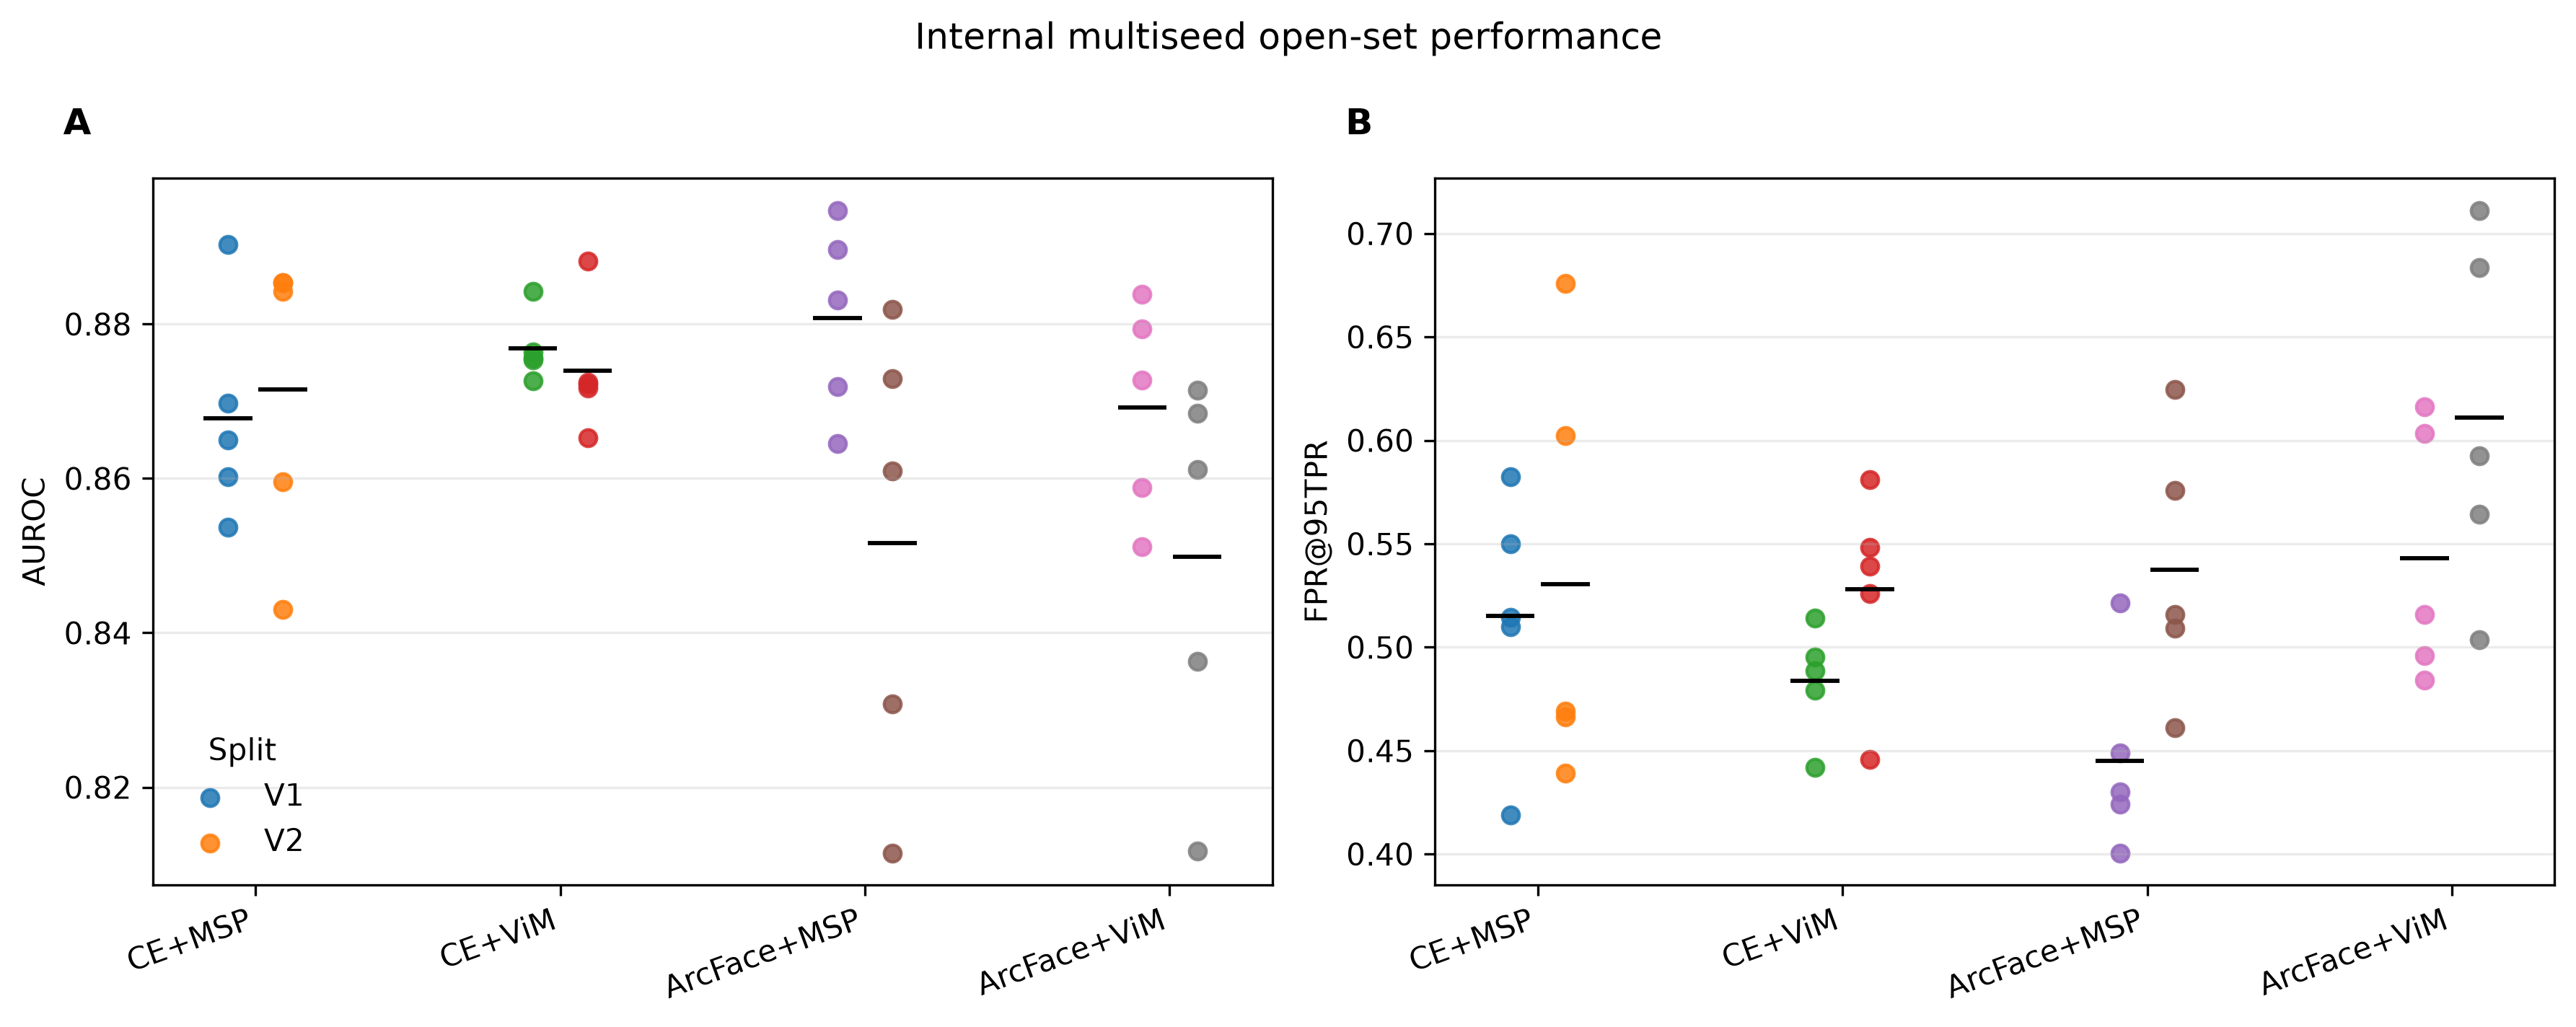
\includegraphics[width=\textwidth]{figures/figure2_internal_performance.png}
\caption{Rendimiento open-set interno en MLL23 sobre cinco semillas.}
\label{fig:interno-es}
\end{figure}

\begin{figure}[htbp]
\centering
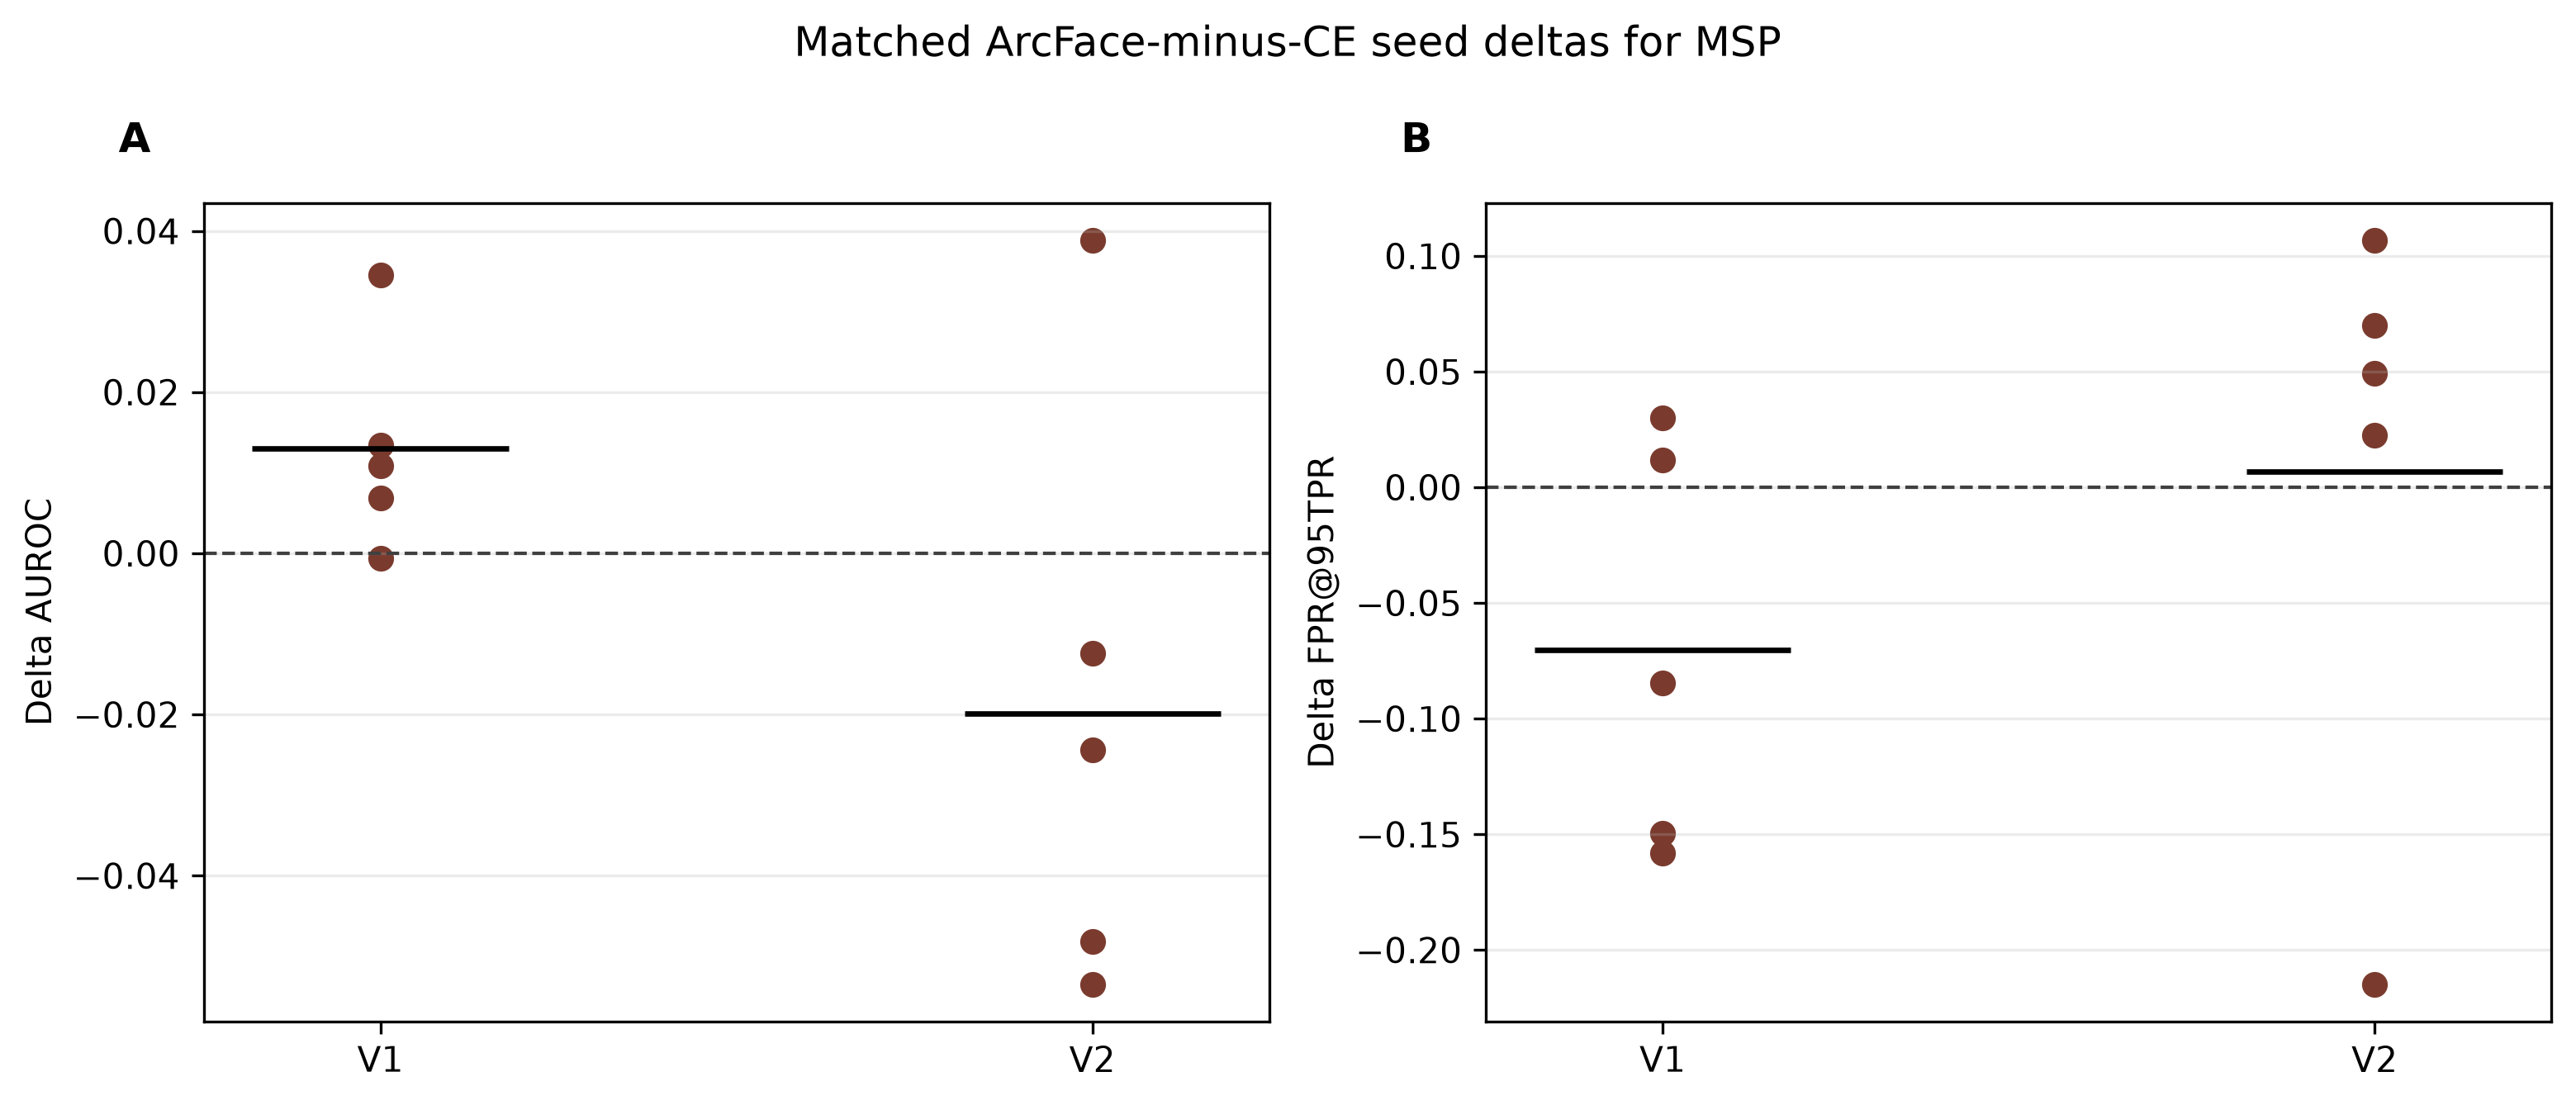
\includegraphics[width=0.9\textwidth]{figures/figure3_arcface_stability.png}
\caption{Deltas pareados ArcFace menos CE para MSP. La tendencia favorable de V1 no se reproduce en V2.}
\label{fig:arcface-es}
\end{figure}

\section{Analisis de Fallos Dependientes de Morfologia}

La dificultad de rechazo desconocido varia fuertemente por morfologia. En el analisis externo CE+ViM, las morfologias desconocidas mas faciles por AUROC medio fueron promielocito (0.897), mielocito (0.880), metamielocito (0.867), promielocito bilobulado (0.856) y eritroblasto (0.792). Las mas dificiles fueron neutrofilo en banda (0.526), monoblasto (0.575), mieloblasto (0.592), linfocito atipico (0.597) y celula sombra (0.782). FPR@95TPR fue particularmente alto para neutrofilo en banda (0.944) y mieloblasto (0.819).

Los fallos se alinean con atractores conocidos. Neutrofilo en banda se predice dominantemente como neutrofilo segmentado; monoblasto como monocito; y mieloblasto, linfocito atipico y celula sombra frecuentemente como linfocito. Esto indica que los errores open-set no son uniformes, sino concentrados en vecindarios morfologicamente plausibles.

\begin{figure}[htbp]
\centering
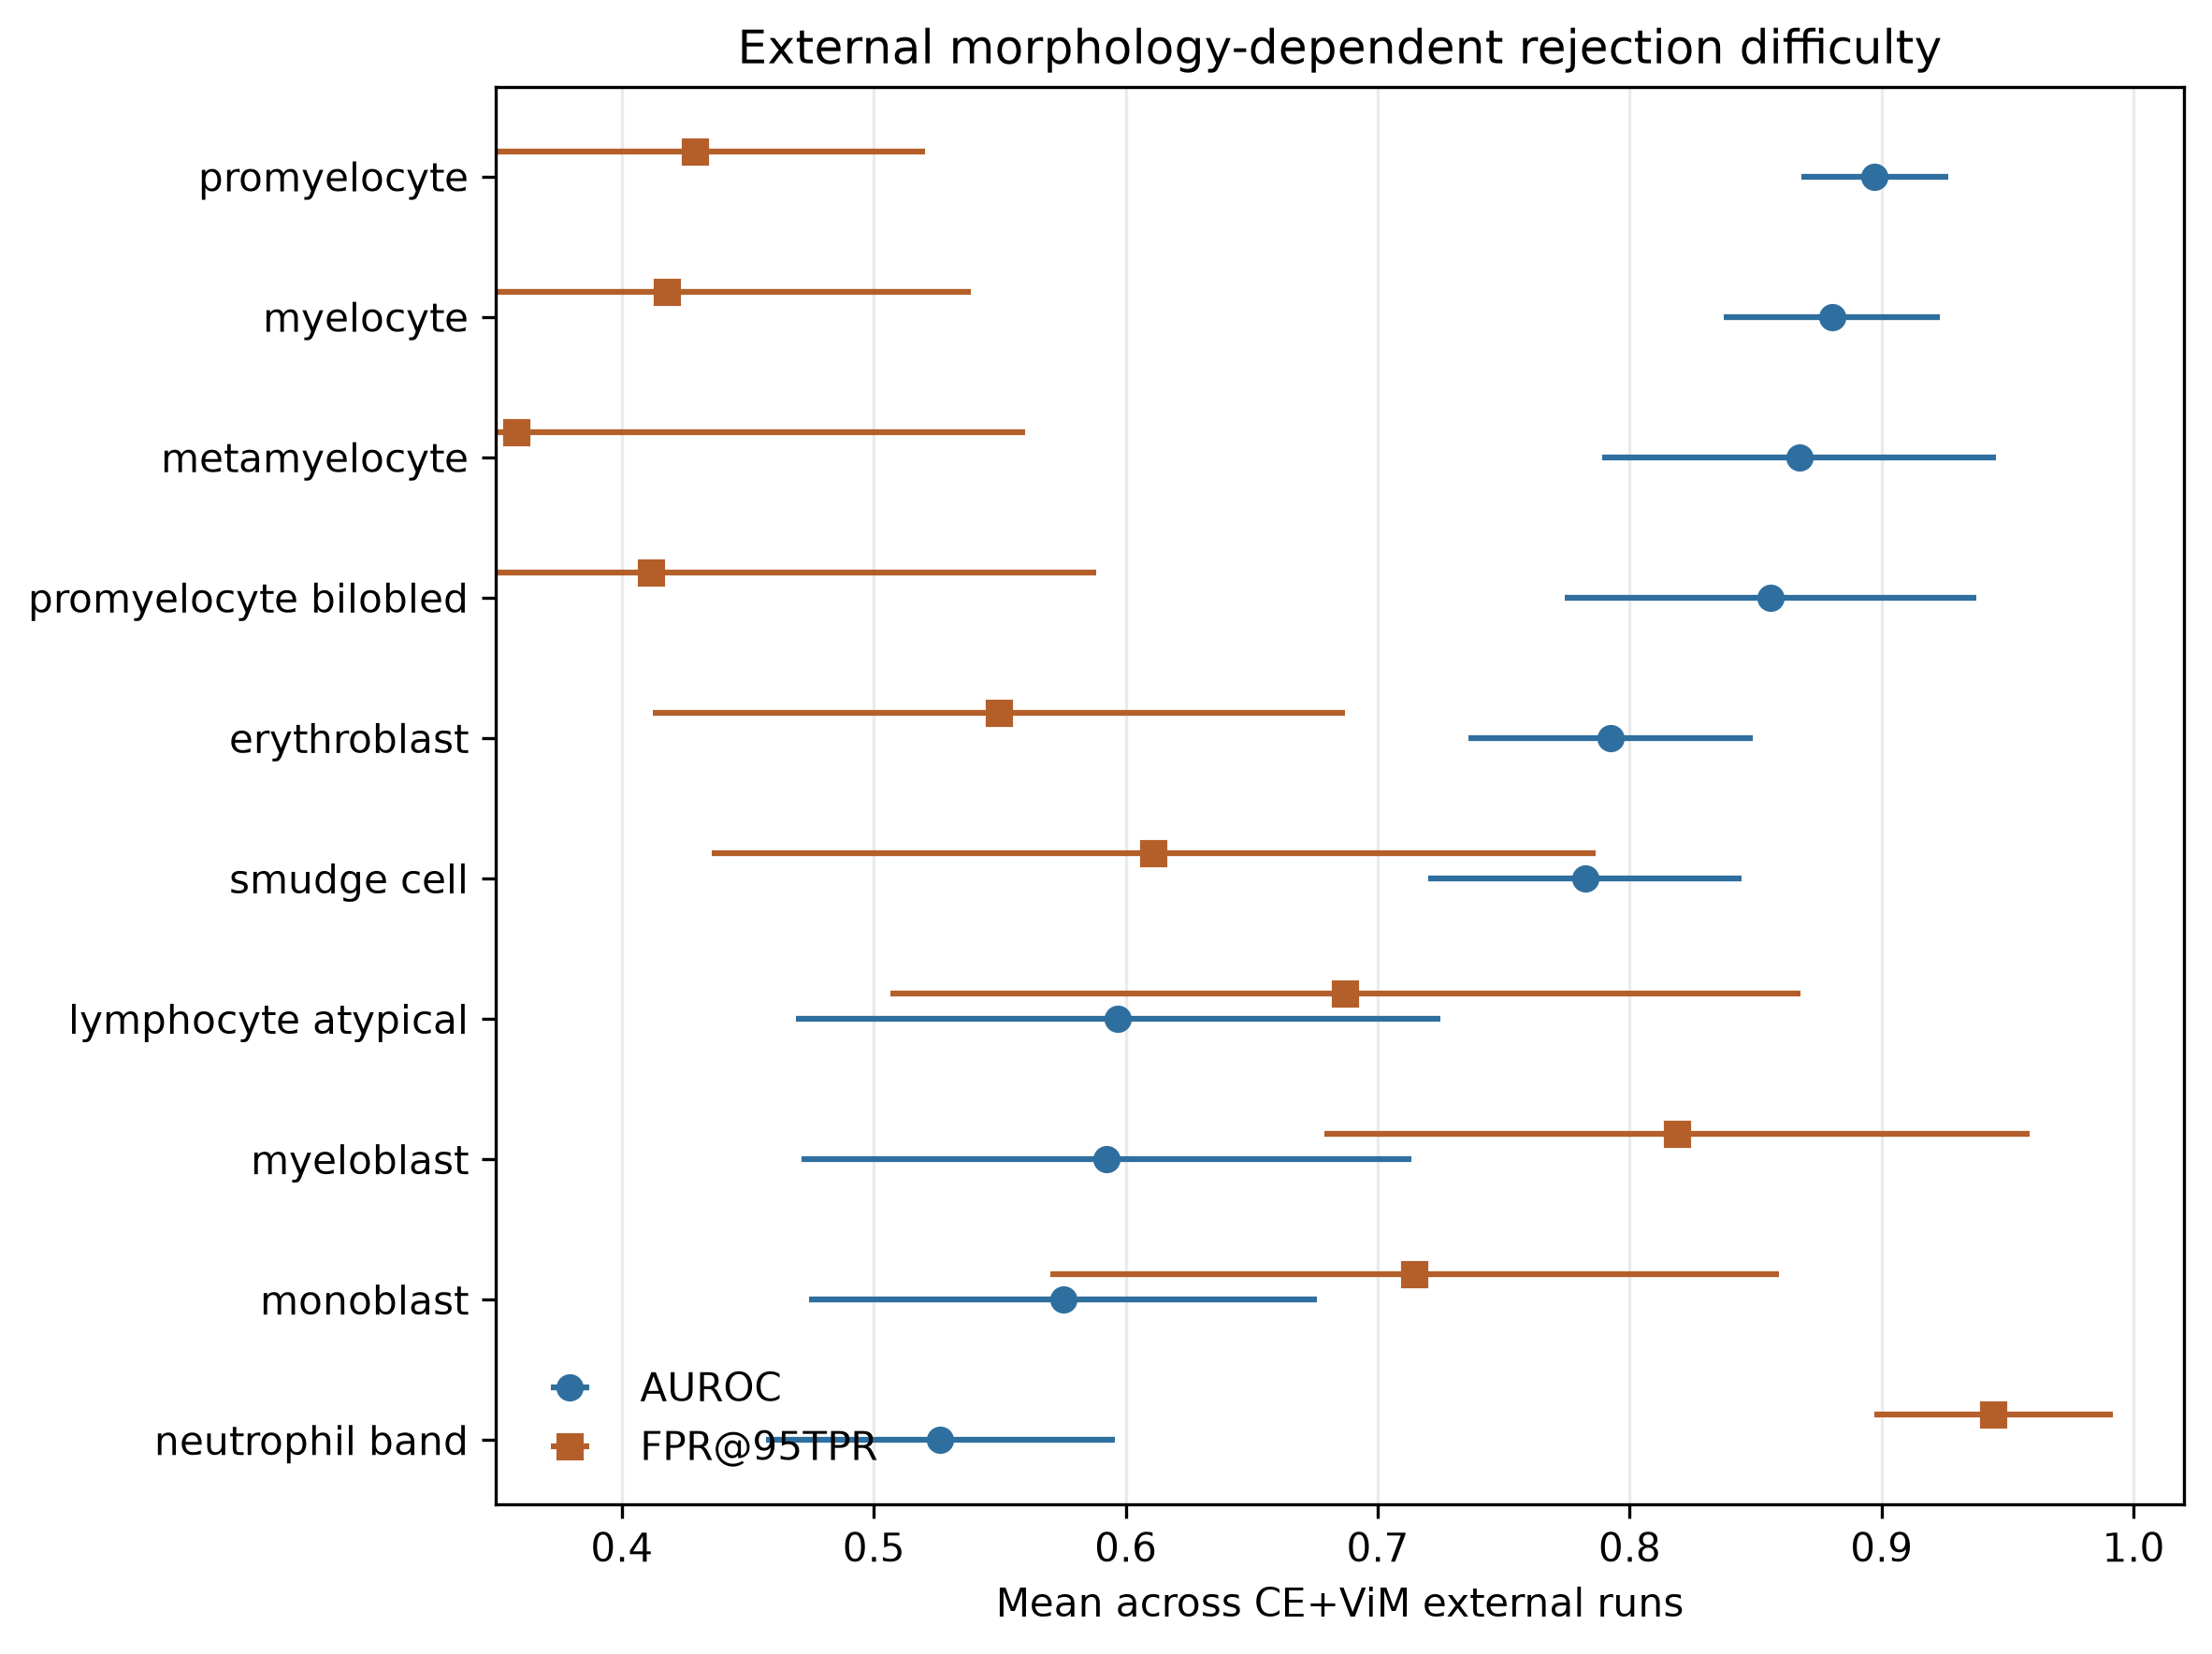
\includegraphics[width=0.86\textwidth]{figures/figure5_external_morphology.png}
\caption{Dificultad externa dependiente de morfologia para CE+ViM.}
\label{fig:morfologia-es}
\end{figure}

\begin{figure}[htbp]
\centering
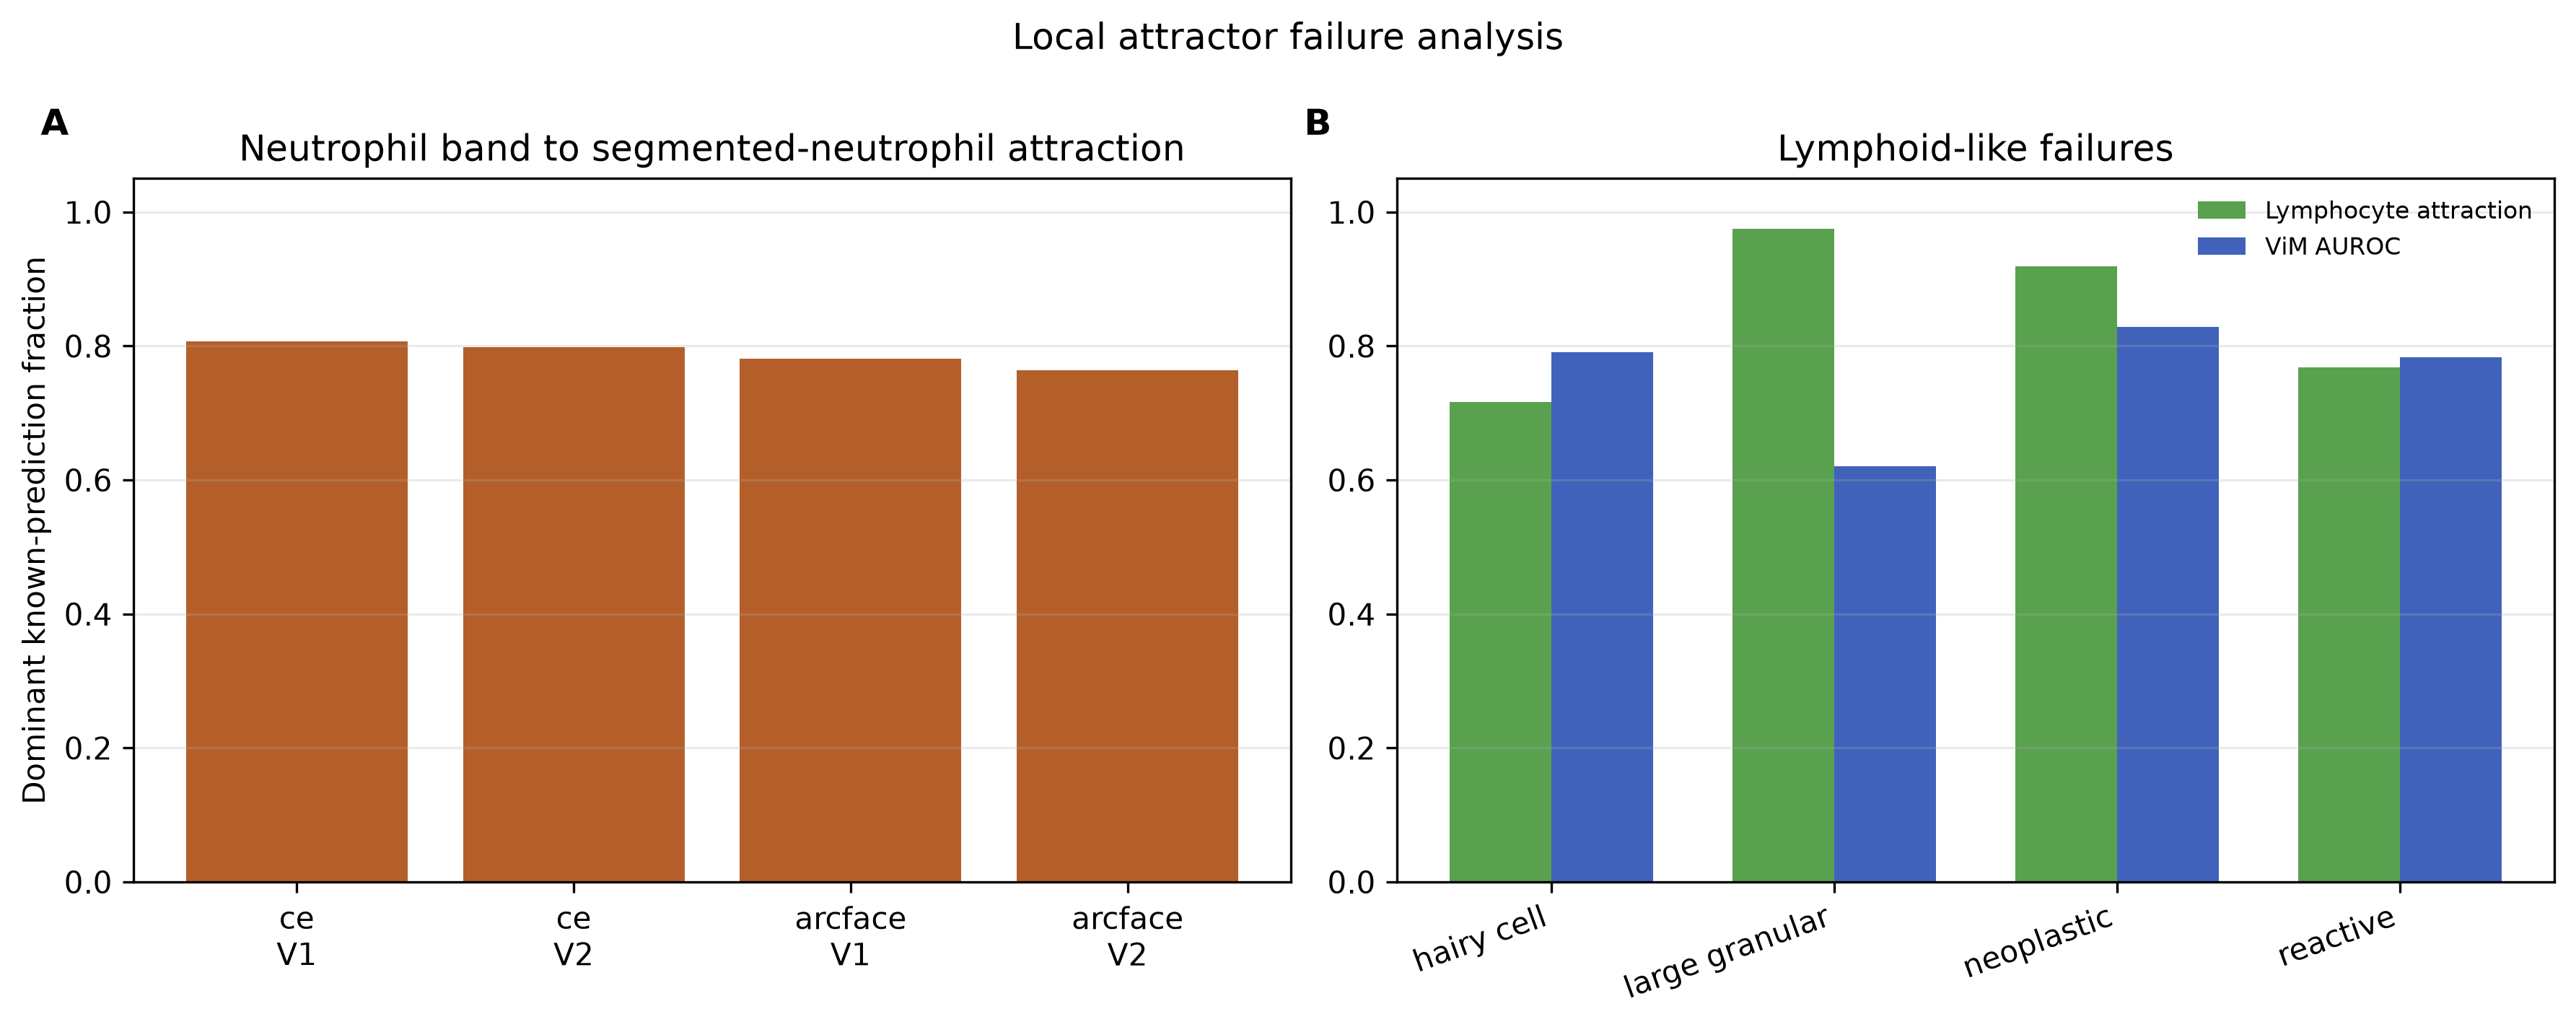
\includegraphics[width=\textwidth]{figures/figure6_failure_cases.png}
\caption{Analisis de atractores hacia clases conocidas para neutrofilo en banda y morfologias linfoides.}
\label{fig:fallos-es}
\end{figure}

\section{Validacion Externa}

AML-LMU es el dominio externo central. Se usa solo despues de congelar modelos, splits, scores y taxonomia. No hay imagenes externas usadas para entrenamiento, ajuste fino, seleccion de score, calibracion de umbral, ajuste de PCA, ajuste de ViM, construccion de bancos kNN ni decisiones de preprocesamiento.

El closed-set externo conserva exactitud aparentemente alta, pero macro-F1 revela degradacion sustancial. V1 ArcFace obtuvo macro-F1 externo 0.755 $\pm$ 0.009, V1 CE 0.711 $\pm$ 0.051, V2 ArcFace 0.708 $\pm$ 0.036 y V2 CE 0.705 $\pm$ 0.030. Todos estan muy por debajo del macro-F1 interno cercano a 0.97.

En OSR externo, V1 CE+MSP obtuvo AUROC/FPR95 0.696 $\pm$ 0.074 / 0.796 $\pm$ 0.134, mientras V1 CE+ViM obtuvo 0.641 $\pm$ 0.090 / 0.785 $\pm$ 0.116. V1 ArcFace+MSP obtuvo 0.690 $\pm$ 0.045 / 0.689 $\pm$ 0.107, y V1 ArcFace+ViM 0.563 $\pm$ 0.084 / 0.879 $\pm$ 0.083. En V2, CE+MSP obtuvo 0.630 $\pm$ 0.094 / 0.887 $\pm$ 0.100; CE+ViM 0.573 $\pm$ 0.123 / 0.867 $\pm$ 0.138; ArcFace+MSP 0.696 $\pm$ 0.069 / 0.723 $\pm$ 0.162; y ArcFace+ViM 0.632 $\pm$ 0.087 / 0.851 $\pm$ 0.062.

El ranking de metodos no se transfirio limpiamente: MSP supero a ViM por AUROC medio externo tanto para CE como ArcFace en V1 y V2. CE+MSP es por ello la linea base practica externa; CE+ViM sigue siendo la linea base interna estable, no el ganador externo.

\begin{figure}[htbp]
\centering
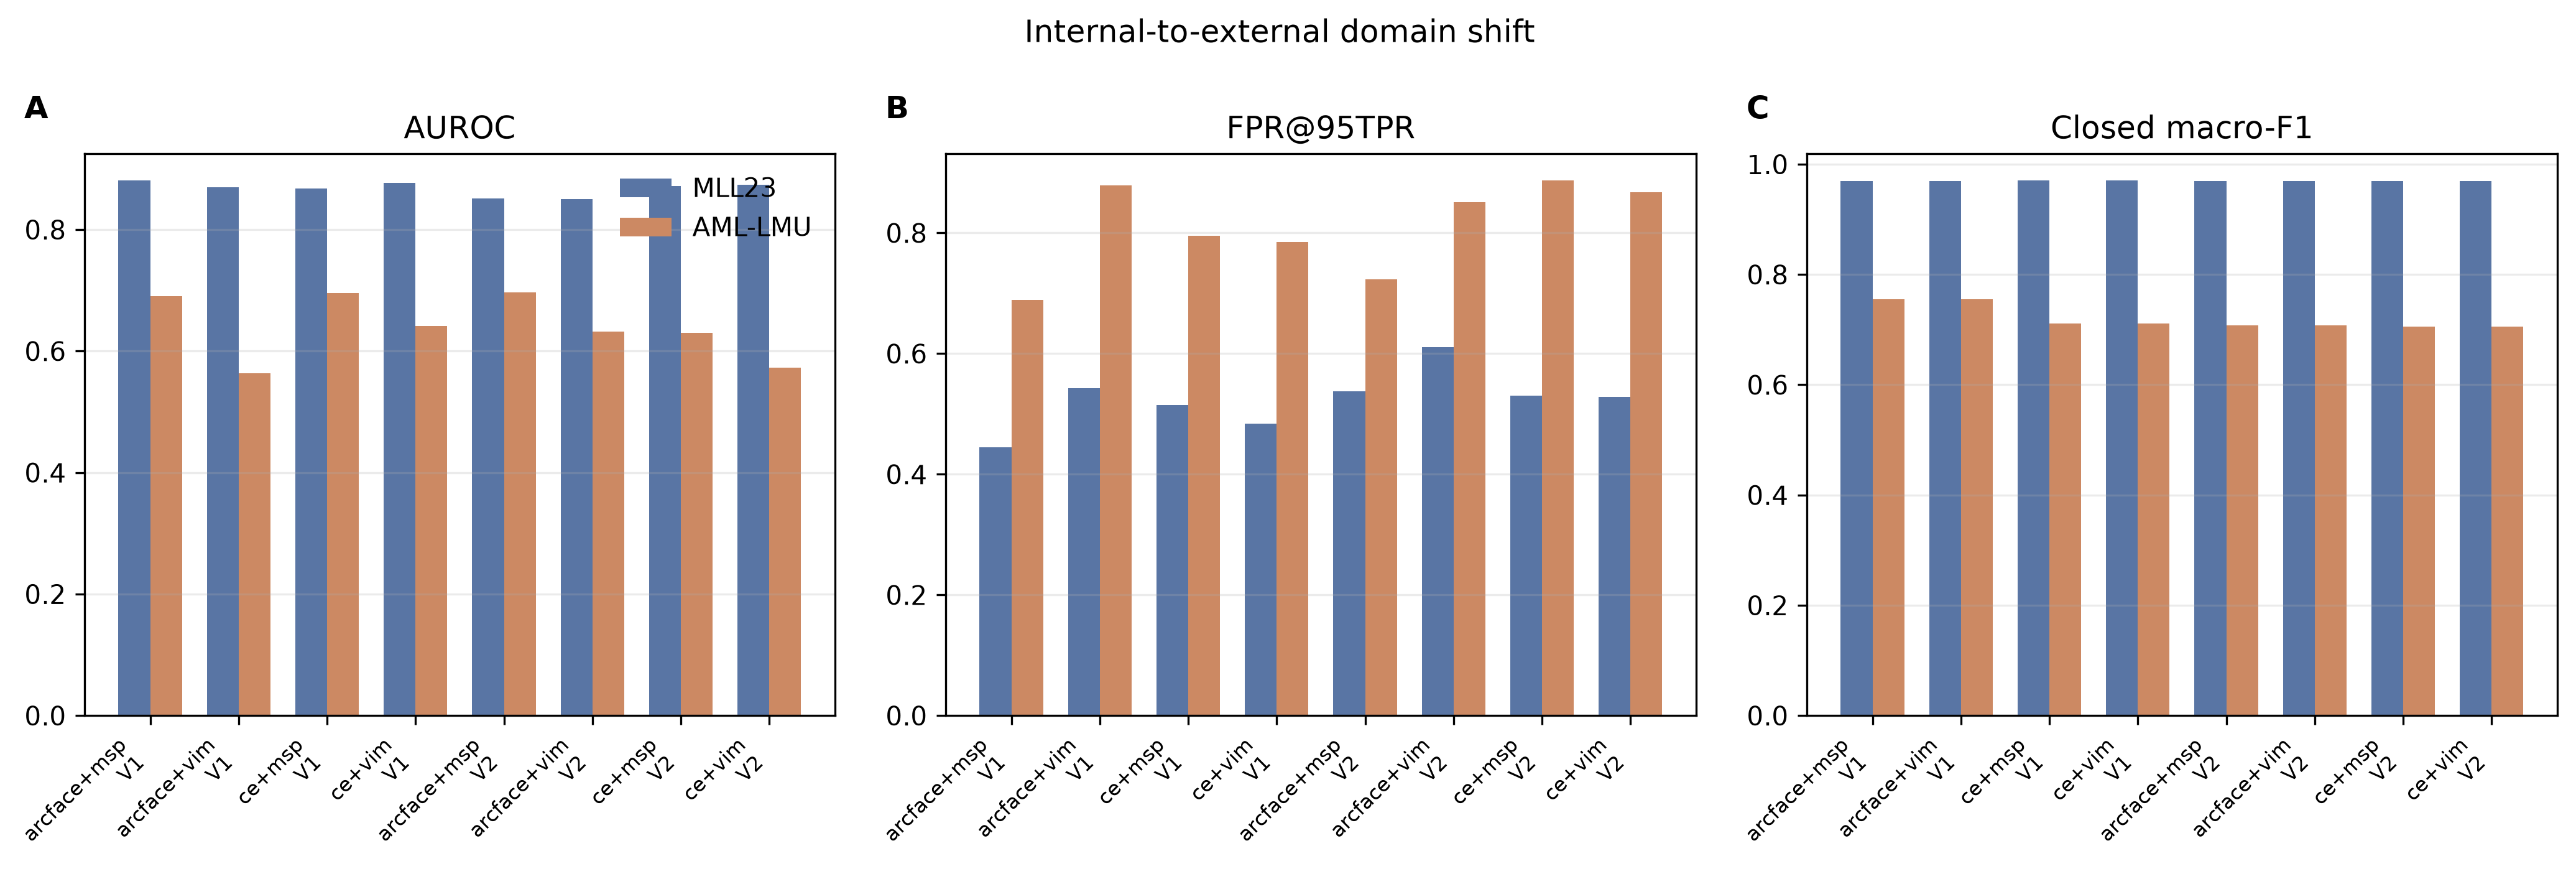
\includegraphics[width=\textwidth]{figures/figure4_domain_shift.png}
\caption{Cambio de dominio interno-externo para sistemas principales.}
\label{fig:dominio-es}
\end{figure}

\section{Analisis Topologico}

La homologia persistente cubical se evaluo como posible representacion predictiva sobre imagenes crudas, mapas morfologicos, candidatos nucleo/citoplasma, mapas de activacion CNN, fusion temprana y fusion tardia. Los resultados no respaldan utilidad predictiva robusta para OSR. TDA-only codifica informacion de clase, con macro-F1 closed-set 0.828 en Delivery 2, pero AUROC open-set queda aproximadamente entre 0.55 y 0.58 para variantes TDA-only, y las fusiones Deep+TDA degradan el baseline profundo principal.

Vietoris-Rips se uso como analisis secundario explicativo. Incluye 500 analisis de nubes sobre MLL23 y AML-LMU, splits V1/V2, representaciones CE/ArcFace, cinco semillas y clases conocidas mas morfologias dificiles predeclaradas. Cada nube tiene resumen H0/H1, para 1,000 filas de homologia. Los resultados son mixtos: H0 suele mostrar mayor variabilidad para ArcFace, pero H1 es debil y las correlaciones topologia--OSR son inconsistentes. Por tanto, VR describe estructura de embeddings, pero no es predictor causal o metodo de deteccion.

\begin{figure}[htbp]
\centering
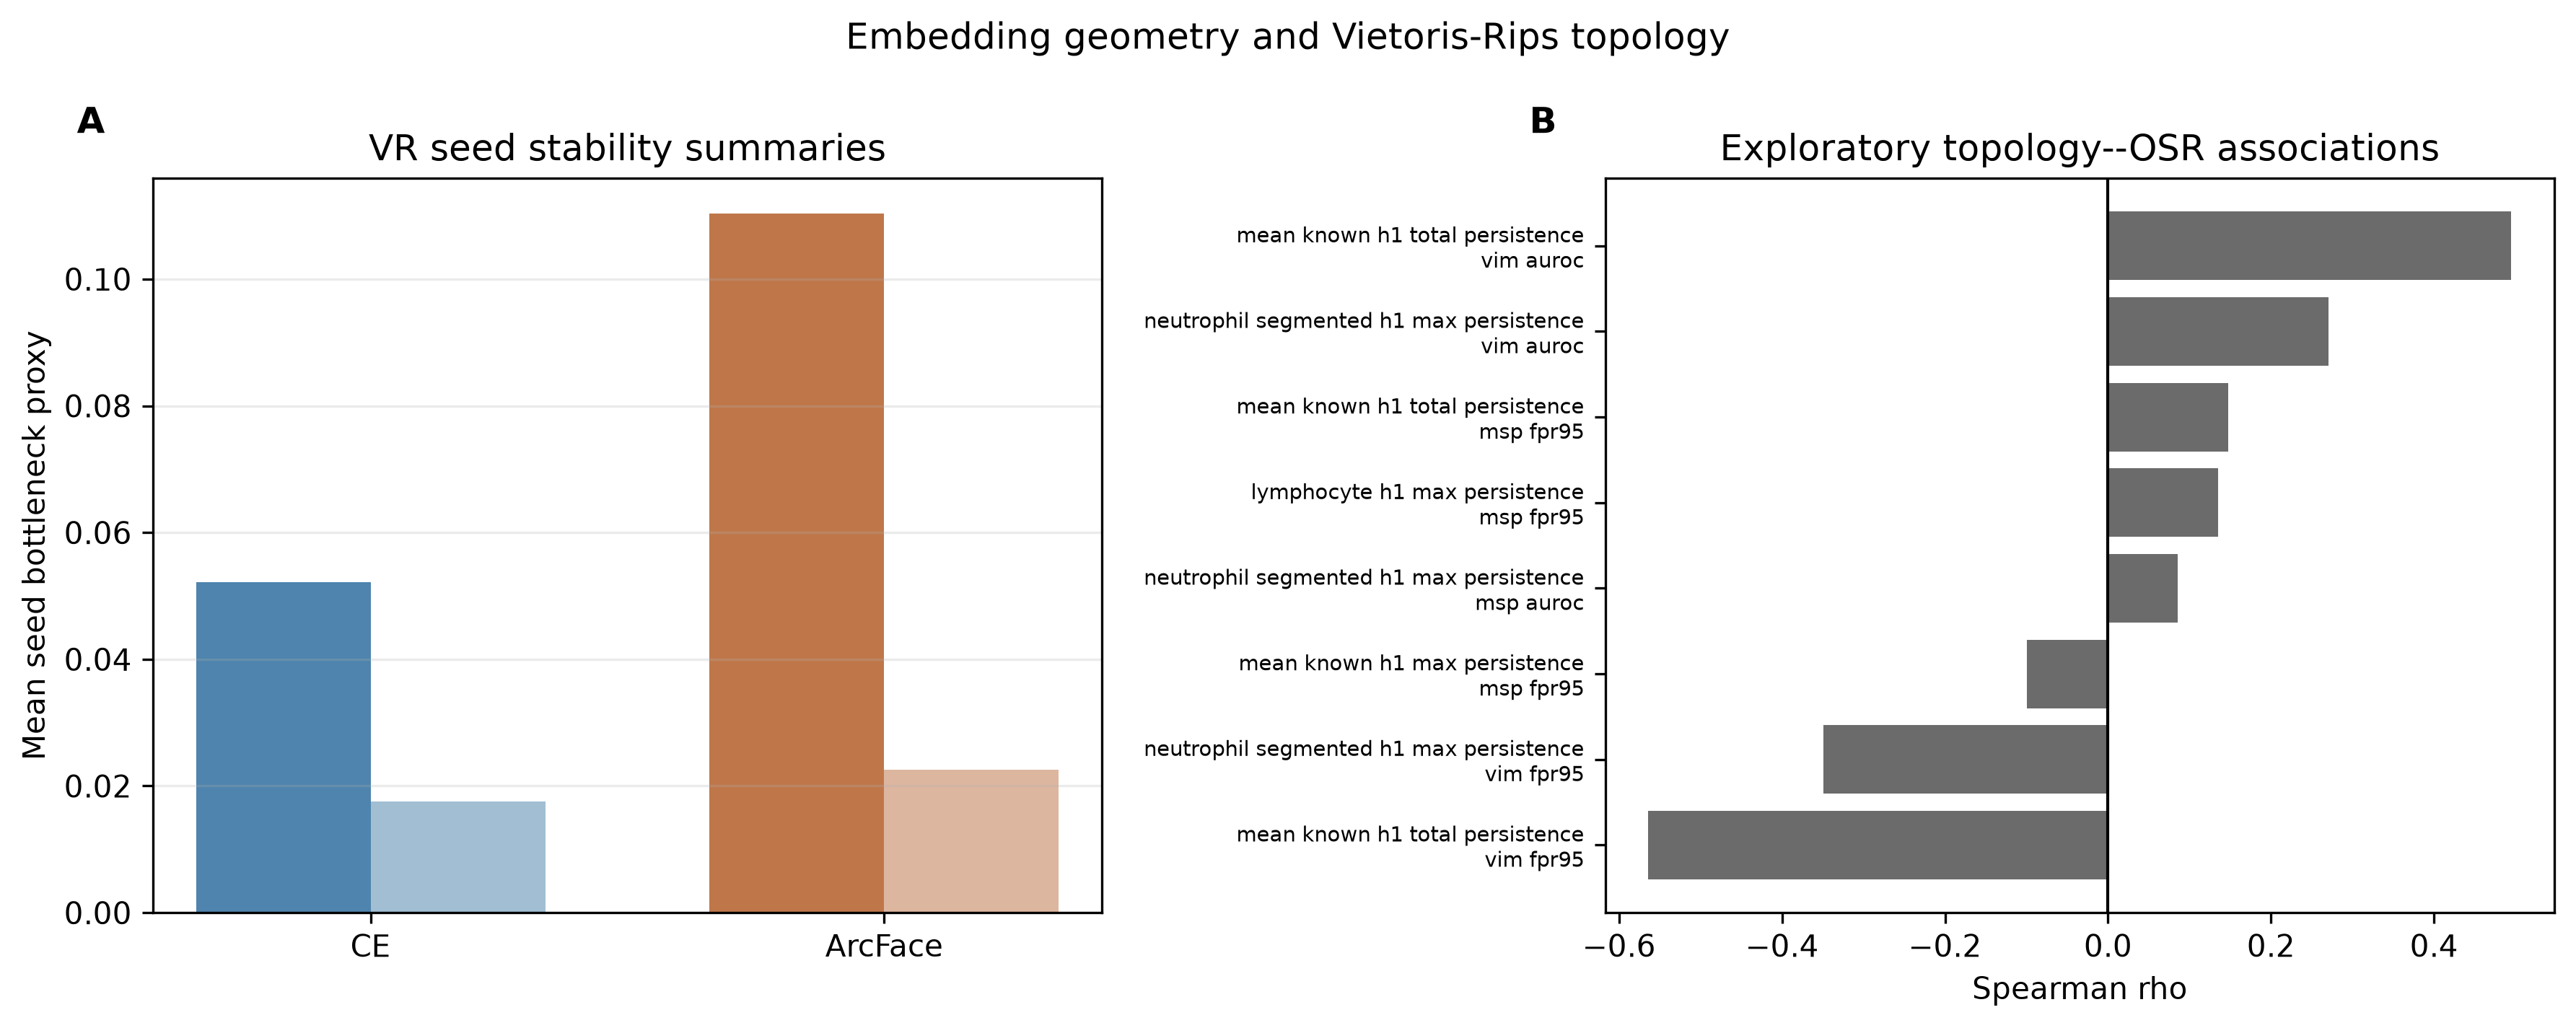
\includegraphics[width=\textwidth]{figures/figure7_topology.png}
\caption{Resumen geometrico y topologico Vietoris-Rips. El analisis es descriptivo, no predictivo.}
\label{fig:topologia-es}
\end{figure}

\section{Discusion}

El resultado principal es que clasificar bien clases conocidas no basta para rechazar morfologias no vistas. Internamente, macro-F1 closed-set cercano a 0.97 convive con FPR@95TPR elevado. Externamente, el cambio de dominio reduce AUROC, aumenta FPR@95TPR y cambia el ranking de scores post-hoc. Esto muestra que la confiabilidad open-set debe evaluarse con semillas multiples, sensibilidad a particiones, validacion externa y analisis por morfologia.

La similitud morfologica aparece como fallo persistente. Neutrofilo en banda se atrae hacia neutrofilo segmentado; monoblasto hacia monocito; y varias morfologias linfoides hacia linfocito. Estas observaciones son de reconocimiento morfologico y no deben leerse como mecanismos biologicos causales ni como afirmaciones diagnosticas.

ArcFace es una ablacion informativa porque mejora algunas metricas de geometria conocida, pero no confirma ganancia open-set robusta. La homologia persistente tambien queda delimitada: cubical PH es una ablacion predictiva negativa rigurosa; Vietoris-Rips es una lente explicativa sobre embeddings, no una evidencia de causalidad topologica.

\section{Limitaciones}

El estudio usa un dominio interno principal y un dominio externo. Los manifiestos no contienen identificadores confiables de paciente/grupo para una separacion paciente-nivel auditada. Las clases desconocidas son definidas por protocolo. Hay fuerte desbalance de clases. La evaluacion multisemilla usa cinco semillas y una familia de backbone ResNet18. ArcFace se evalua con una sola configuracion congelada de escala y margen. El conjunto desconocido interno fue inspeccionado durante entregas previas, por lo que los analisis internos posteriores no son descubrimiento independiente. No se realiza adaptacion externa, lo que fortalece la prueba test-only pero no evalua metodos domain-adaptive.

\section{Conclusion}

Este articulo presenta una evaluacion disciplinada de reconocimiento open-set para morfologias hematologicas no vistas. La leccion central es que el desempeno closed-set alto no implica rechazo confiable de desconocidos. ArcFace mejora algunas propiedades geometricas, pero no se reproduce como representacion superior robusta. La homologia persistente cubical funciona como ablacion predictiva negativa, y Vietoris-Rips aporta descripcion de embeddings sin justificar un claim causal. La validacion externa AML-LMU muestra degradacion en todos los sistemas principales y cambio en el ranking de metodos post-hoc. El resultado defendible es que la confiabilidad open-set hematologica es afectada por similitud morfologica, estabilidad de representacion y cambio de dominio de adquisicion.

\bibliographystyle{plain}
\bibliography{references}

\end{document}
